\section{INTRODUCTION}

Consider an on-call engineer's agent investigating a production incident: it can query metrics, logs, traces, the deployment history, a ticketing system and internal documentation, all through MCP. If it calls every one of those tools for every question, retrieves each response in full, and hands the result to the model unfiltered, the resulting prompt may run to thousands of tokens, most of it irrelevant to the specific question asked, with the one line that explains the incident potentially buried in the middle of a long log dump. This is not a hypothetical: it is the default behavior of an MCP agent with no context-governance layer, and it is the behavior this paper measures directly against a governed alternative.

Once an LLM agent has access to many Model Context Protocol (MCP) tools, it may call more of them than necessary, retrieve excessive raw output, duplicate context across steps, and pass noisy or weakly relevant evidence into the model. The result is a quality-efficiency problem: the agent becomes slower, more expensive, and harder to audit, without a corresponding gain in answer quality. MCP standardizes tool connectivity; it does not decide which tools are necessary, how much of each tool's output should be retained, how heterogeneous outputs should be compressed, or how retained evidence should be ordered so the model uses it effectively.

This problem connects directly to several established research streams. MCP standardizes access to tools and external data sources \cite{Anthropic2024, MCP2025}, while recent MCP analyses map its lifecycle and security implications \cite{Hou2025}. Retrieval-augmented generation and self-reflective retrieval show the value of grounding answers in external evidence \cite{Lewis2020, Asai2024}, and long-context research shows that simply placing relevant information in a prompt does not guarantee that the model will use it effectively \cite{Liu2024a}. PR-SC MCP builds on these foundations by focusing on the context lifecycle after tool access: which evidence is selected, compressed, attributed, ordered and measured once multiple tools have returned heterogeneous outputs.

This paper argues that scalable MCP-based agents require an explicit context-engineering layer and proposes PR-SC MCP: a context control-plane architecture combining predictive routing, source-aware compression, evidence packaging and observability feedback. The central research question is whether disciplined context governance can materially reduce token burden, tool calls and latency without degrading answer quality, evidence retention or robustness, and whether that trade-off holds up once the pipeline is evaluated against a live LLM rather than only deterministic proxies.

The study contributes a comprehensive context-governance architecture for MCP-based agents, a controlled evaluation design that isolates routing, compression, packaging and robustness mechanisms, a live-generation validation matrix spanning three open-weight models under a shared runner, a run-level statistical interpretation with confidence intervals, and a semantic review calibration sample. These contributions draw on tool-augmented reasoning, retrieval, compression, long-context and agent-evaluation research, but apply those ideas to a specific MCP problem: governing heterogeneous tool outputs as an auditable evidence lifecycle rather than treating context as an accumulated prompt. Together, these contributions position PR-SC MCP as both an architectural proposal and an evaluation methodology for measuring whether MCP agents can reduce unnecessary context while preserving source attribution, uncertainty handling, failure-mode discipline and reviewed semantic answer quality.

This decomposes into six sub-questions spanning tool-selection efficiency, compression and evidence retention, evidence packaging and salience, the quality-efficiency trade-off, robustness under adverse conditions, and evaluation validity under live generation. These sub-questions are evaluated through seven hypotheses tied one-to-one to these mechanisms across both validation stages rather than a single benchmark.

\section{THE PR-SC MCP ARCHITECTURE}

PR-SC MCP treats context as an actively governed resource rather than a passive accumulation of tool outputs. This design follows from the broader context-engineering view that model inputs should be deliberately selected, transformed and structured rather than merely expanded \cite{Mei2025}.

The architecture processes context through a sequential pipeline: first, a user query is interpreted for intent and evidence needs. A Tool-Server Capability Index and a predictive routing layer then select a minimum viable toolset instead of calling every connected server. Next, selected tools execute under context budgeting, and their raw outputs pass through source-aware parsing and compression, which apply different strategies to structured, semi-structured, and unstructured sources while preserving decision-relevant content. Retained evidence is subsequently recorded in an evidence ledger that tracks provenance, required-or-optional status, and freshness. Following this, an anti-lost-in-the-middle packaging step orders evidence for salience before constructing the final prompt. Finally, an observability feedback loop logs tokens, tool calls, latency, and quality signals for every run, closing the loop for auditability and tuning.

\subsection{Design Principles}

Table \ref{tab:principles} summarizes the seven design principles that guide every architectural decision described in the remainder of this section.

\begin{table*}[!t]
  \caption{The seven design principles underlying PR-SC MCP.}
  \label{tab:principles}
  \begin{tabular}{p{0.28\linewidth}p{0.62\linewidth}}
    \toprule
    \textbf{Principle} & \textbf{Statement} \\
    \midrule
    1. Context is a managed resource & Every token has cost, latency, and attention implications; context must be selected, parsed, compressed, and ordered deliberately, not accumulated. \\
    2. Tool access should be minimal but sufficient & The architecture identifies the minimum viable toolset needed to answer faithfully, rather than assuming more tools is always better. \\
    3. Routing requires a capability index & A predictive router needs an explicit map of which MCP servers and tools provide which evidence types, not a purely prompt-level guess. \\
    4. Compression must be source-aware & Logs, metrics, traces, diffs, tickets, documentation, and security findings cannot share one generic compression strategy. \\
    5. Evidence must remain attributable & A final answer must be traceable back to the tools that supported it; the evidence ledger records what was called, retained, compressed, and packaged. \\
    6. Ordering affects usability & Evidence position is an architectural decision: important evidence is placed to increase salience and reduce lost-in-the-middle risk. \\
    7. Context decisions must be observable & Tool count, tokens, latency, evidence retention, recall, truncation, and readiness gates must be measurable, or optimization cannot be evaluated. \\
    \bottomrule
  \end{tabular}
\end{table*}

\begin{figure*}[!t]
\centering
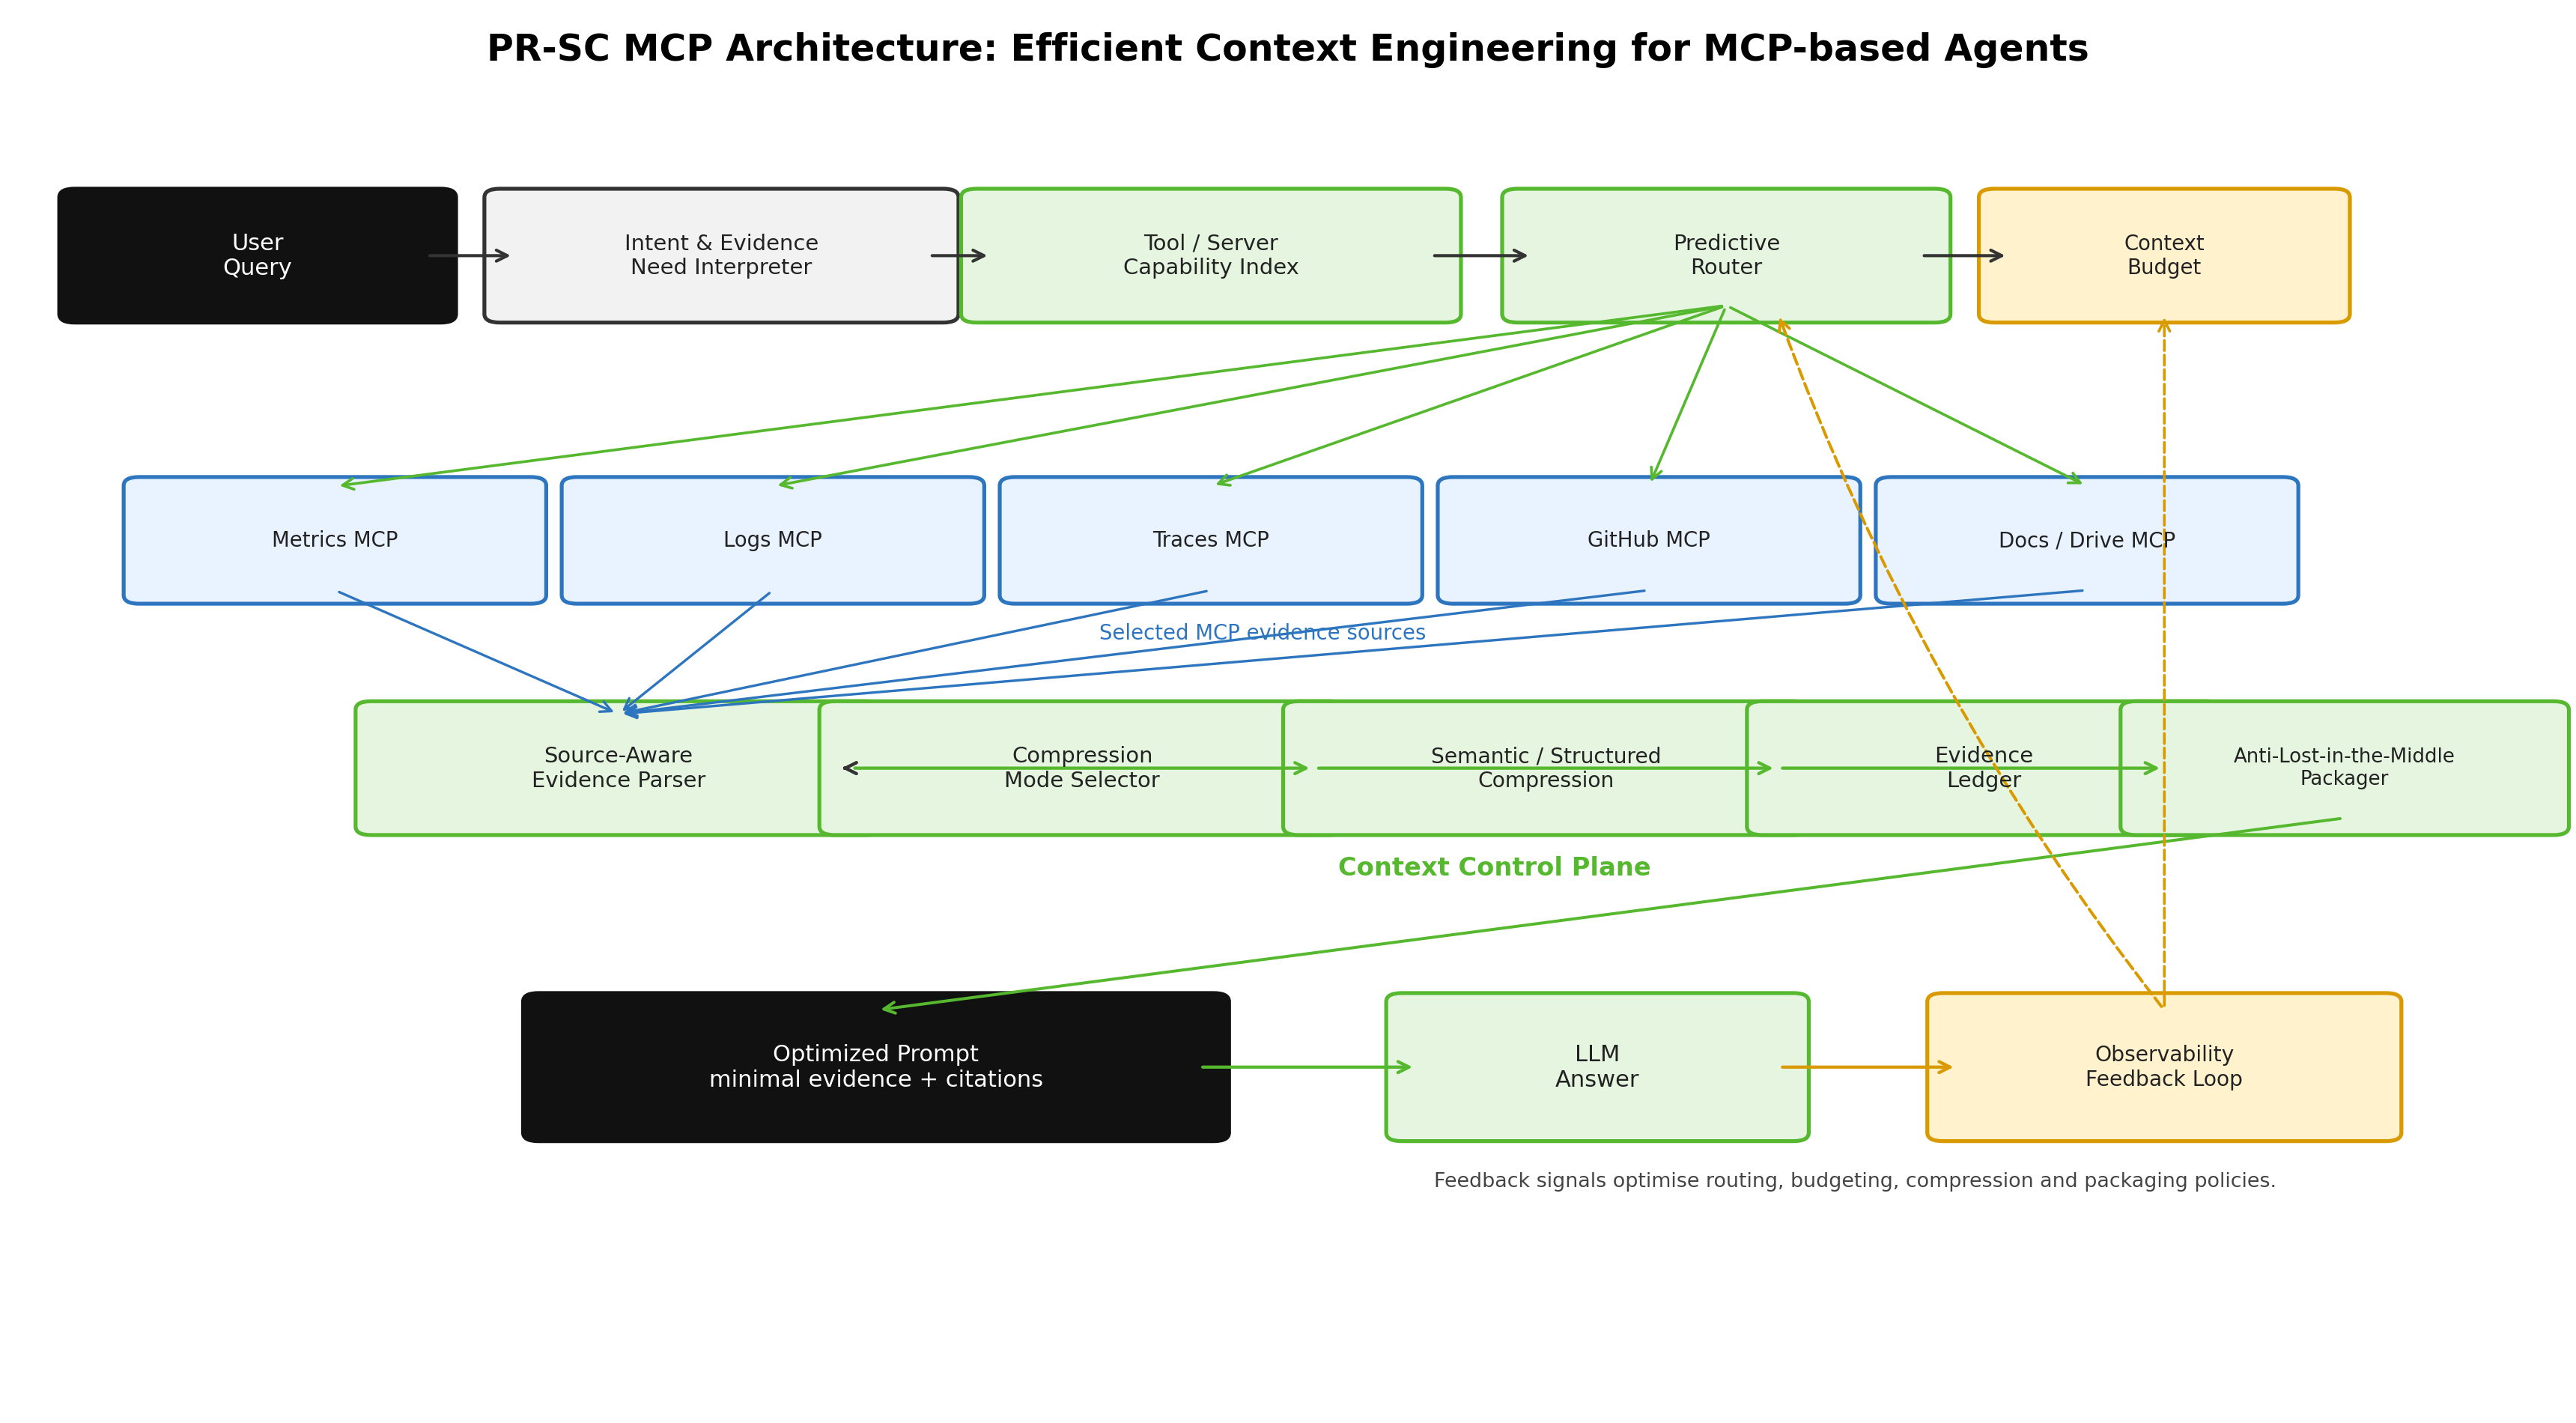
\includegraphics[width=0.85\linewidth]{images/architecture.png}
\caption{PR-SC MCP architecture: query interpretation, predictive routing, source-aware compression, evidence ledgering and packaging, and the observability feedback loop.}
\label{fig:architecture}
\end{figure*}

Figure \ref{fig:architecture} shows this pipeline end-to-end, from the initial query through routing, compression, ledgering and packaging to the observability feedback loop. Four properties differentiate this from exhaustive MCP usage and from traditional RAG. Relative to exhaustive MCP, PR-SC MCP adds tool selection discipline, compression, provenance tracking, and ordering---exhaustive usage typically calls all available tools and forwards raw output with limited control. Relative to traditional RAG, PR-SC MCP is designed for heterogeneous, frequently changing, tool-shaped evidence (logs, traces, diffs, tickets, security signals) rather than a static document corpus, and it treats every tool output as an attributable, potentially adversarial artifact rather than as pre-vetted context.

\subsection{Predictive Routing}

Before any tool executes, an Intent and Evidence-Need Interpreter classifies the user query and estimates which evidence types are plausibly required. A Tool-Server Capability Index describes what each connected MCP server can provide, and a predictive routing layer scores candidate tools against the estimated evidence need, selecting a minimum viable toolset under an explicit context budget rather than calling every available server. This is the mechanism most directly responsible for the tool-count reductions reported in the Results section, and it is motivated by tool-augmented and API-selection work. Toolformer and ReAct establish tool use as a learnable and operationally useful capability \cite{Schick2023, Yao2023}, while Gorilla shows the importance of selecting the right API from a large and overlapping catalog \cite{Patil2024}. PR-SC MCP applies that motivation at the MCP server-tool level, where routing is one component of a broader context-governance pipeline rather than the full contribution.

\subsection{Source-Aware Compression}

Selected tools execute through an MCP Tool Execution Layer, and their raw outputs pass through source-aware parsing before compression. Parsing is source-specific: logs, traces, repository diffs, tickets and documentation have different structures and different signals worth preserving, so a single generic summarization strategy is deliberately avoided. A compression-mode selector then chooses between semantic and structured compression depending on the source type, aiming to reduce token volume while preserving the specific facts, thresholds, and identifiers a downstream answer will need to cite. Structured compression applies to sources with a regular schema, such as metrics and traces, where fields, timestamps and thresholds are extracted and retained verbatim while redundant formatting is dropped; semantic compression applies to free-text sources, such as tickets and documentation, where a summarization step condenses prose while flagging named entities and numeric values as protected spans that must survive compression unchanged. This layer draws on prompt-compression and retrieval-compression research \cite{Jiang2023, Jiang2024, Xu2024}, but applies the idea to heterogeneous MCP tool outputs. The purpose is not only to shorten context, but to preserve source-specific evidence such as identifiers, thresholds, timestamps, diffs and diagnostic signals that may be lost under generic compression.

\subsection{Evidence Ledger and Anti-Lost-in-the-Middle Packaging}

Every piece of retained evidence is recorded in an evidence ledger that tracks its source tool, its required-or-optional status, and a freshness signal, so that later stages and subsequent human review can trace any claim in the final answer back to the tool call that produced it. Concretely, each ledger entry stores the originating tool name, a timestamp, the compression mode applied, and a required-or-optional flag inherited from the routing decision that selected it, so that a reviewer can reconstruct not only what evidence was used but why it was considered necessary. The contribution of this layer is not merely that context is reduced, but that it is made traceable and auditable: every claim in a final answer must be linkable back to a specific ledger entry, and the ledger itself is what allows the architecture to distinguish required evidence from optional, stale, conflicting, or potentially adversarial evidence, rather than treating all retained context as equally trustworthy. An anti-lost-in-the-middle packaging step then orders this evidence for salience before constructing the final prompt, directly addressing the finding that models can fail to use evidence buried in the middle of long contexts \cite{Liu2024a}. Packaging is accordingly not a generic ordering step; it is a deliberate evidence-presentation strategy intended to prevent the most decision-relevant evidence from being buried in the middle of the prompt, where a model is least likely to use it. Beyond architectural positioning, this framework integrates adversarial-agent research showing that retrieved or tool-supplied content can carry harmful instructions or misleading claims \cite{Greshake2023, Zhan2024, Radosevich2025}. For this reason, PR-SC MCP treats tool output as attributable and potentially untrusted evidence by default, rather than as neutral prompt text.

\subsection{Observability Feedback Loop}

An Optimized Prompt and LLM Generation layer constructs the final prompt from the packaged evidence and produces the answer. Subsequently, an observability feedback loop logs tokens, tool calls, latency, finish reason, and quality signals for every run. This granular observability enables the token-accounting analysis presented in Section 4.3; without per-run visibility into prompt and output token counts across repeated runs, the run-to-run stability of the efficiency result under live generation could not be definitively established. The same logs are also what make the run-level statistical treatment in Section 4.4 possible in the first place, since paired comparisons between variants require every run to be individually attributable to a specific case, variant, and model. Concretely, the observability log is what allows every table in Section 4 to be reproduced from raw run data, what supports the paired Full-versus-Exhaustive comparisons underlying Table \ref{tab:ci}, and what makes it possible to determine whether an observed latency improvement is attributable to reduced context size or to model-specific generation behavior, rather than to an unexamined confound between the two.

The observability layer distinguishes prompt tokens, completion tokens and total tokens. Prompt tokens capture the architecture-controlled context burden, whereas total tokens capture the end-to-end live-generation footprint, including both the constructed prompt and the model-generated completion.

\subsection{End-to-End Flow}

A single query moves through nine steps: (1) the intent and evidence-need interpreter classifies the query; (2) the Tool-Server Capability Index and predictive router select a minimum viable toolset under a context budget; (3) the selected tools execute through the MCP Tool Execution Layer; (4) raw outputs pass through source-aware parsing; (5) the compression-mode selector chooses a semantic or structured strategy per source; (6) retained evidence and its provenance are written to the evidence ledger; (7) the anti-lost-in-the-middle packager orders evidence for salience; (8) the optimized prompt is constructed and sent to the model; and (9) the observability feedback loop logs the run and feeds the routing, budgeting, compression, and packaging policies for subsequent queries. Steps 2, 4--5, 6--7 and 9 correspond respectively to Sections 2.2, 2.3, 2.4 and 2.5 above. Because each step writes to the evidence ledger or the observability log, a failure at any point in this flow is attributable to a specific step rather than surfacing only as an incorrect final answer, which is the property that Section 3.1 relies on to make benchmark failures decomposable.

\subsection{Architecture Variants Compared in This Study}

Section 4 reports results for eight architectural variants. Three serve as external baselines representing pre-existing or exhaustive approaches; the remaining five constitute systematic ablations of PR-SC MCP's core mechanisms. The three baselines are chosen to represent distinct, already-established ways of handling context rather than a single strawman: Exhaustive MCP represents the uncontrolled default behavior of an MCP agent with no governance layer, Traditional RAG represents a static, retrieval-centric alternative predating MCP, and Direct Long-Context represents the simplest possible response to context growth, namely relying on a larger context window instead of active governance. The five ablation variants then isolate PR-SC MCP's own mechanisms against this backdrop: each one selectively toggles routing, compression, and packaging on or off, so that their individual and combined contributions can be attributed rather than inferred from the full architecture alone. Table \ref{tab:variants} defines the precise operational parameters of each variant.

\begin{table*}[!t]
  \caption{The eight architecture variants compared during Architecture Validation and their relationship to PR-SC MCP's four mechanisms. Live Validation (Sections 4.2--4.6) narrows this to the four variants that survived as most diagnostic: Exhaustive MCP, Routing MCP, Routing + Packaging, and Full PR-SC MCP.}
  \label{tab:variants}
  \begin{tabular}{p{0.22\linewidth}p{0.72\linewidth}}
    \toprule
    \textbf{Variant} & \textbf{What it does} \\
    \midrule
    Exhaustive MCP & Calls every connected MCP tool for each query and forwards raw, uncompressed output directly into the prompt. No routing, compression, packaging or ledger---the uncontrolled baseline. \\
    Traditional RAG & Replaces live MCP tool calls with retrieval from a static, pre-indexed document corpus, following the classic RAG pattern; a pre-MCP, retrieval-centric alternative rather than a PR-SC MCP ablation. \\
    Direct Long-Context & Passes a large, undifferentiated block of raw source data directly to the model with minimal governance, testing whether context length alone can substitute for a governance layer. \\
    Compression-only MCP & Calls all tools, unrouted, but compresses their output before inclusion---isolates the effect of compression without better tool selection. \\
    Routing MCP & Applies predictive routing to select a minimum viable toolset but performs no compression or packaging---isolates the effect of routing alone. \\
    Routing + Compression, no packaging & Combines routing and compression but does not reorder evidence for salience. \\
    Routing + Packaging, no compression & Combines routing and evidence packaging but skips compression. \\
    Full PR-SC MCP & Applies routing, source-aware compression, evidence ledgering and anti-lost-in-the-middle packaging together, with the observability feedback loop active throughout. \\
    \bottomrule
  \end{tabular}
\end{table*}

\section{EVALUATION APPROACH}

The architecture is evaluated in two stages rather than once. The first stage, Architecture Validation, tests the eight variants defined in Table \ref{tab:variants} under controlled and semi-real conditions with deterministic scoring, so that routing, compression and packaging can be isolated and measured without the added variability of live model generation. The second stage, Live Validation, takes the most diagnostic variants from the first stage and tests them against a live LLM, then checks the result for replicability and provider-generality. This ordering matters: a weakness in the deterministic scoring would be invisible if the first live run were treated as the only evidence, and a live-generation artifact would be invisible without a controlled baseline to compare it against.

The evaluation design is informed by two complementary benchmark traditions. RAGAs motivates reference-free evaluation dimensions such as faithfulness and context precision for retrieval-augmented systems \cite{Es2024}, while AgentBench and MCP-AgentBench motivate agent evaluation across multi-step and tool-mediated settings \cite{Liu2024b, Guo2026}. This study adopts a targeted, mechanism-focused design: instead of maximizing the breadth of servers or tasks, it repeatedly evaluates controlled diagnostic case families across architecture variants and live models, allowing token accounting, latency effects, robustness behavior and human semantic review to be analyzed together.

\subsection{Architecture Validation Design}

\begin{sloppypar}
Twenty-four benchmark cases were constructed against enterprise-style operational evidence: metrics, logs, traces, repository diffs, tickets, documentation and security signals drawn from a simulated observability environment spanning services such as checkout-api, auth-gateway and a reporting pipeline. Each case is defined by a structured schema: the user query, the expected answer, required and optional tools, an explicit list of irrelevant tools, ground-truth evidence fragments that must be retained, distractor evidence that must not be treated as causal, and an expected uncertainty statement for cases with incomplete evidence. This schema makes failure decomposable: if a variant answers incorrectly, the case design identifies whether the failure occurred during tool selection, compression, evidence linkage, packaging or answer generation, rather than leaving the failure as an unexplained wrong answer.
\end{sloppypar}

Twelve failure modes were deliberately injected across the case set (Table \ref{tab:failuremodes}), so that the benchmark tests not only efficiency but whether the architecture behaves safely when tool output is incomplete, stale, malformed, conflicting or noisy---the operational conditions a production MCP agent will eventually meet.

The injected failure modes also reflect lessons from adversarial and robustness work on tool-integrated agents. Indirect prompt injection demonstrates that retrieved content, not only user input, can contain instructions a model may follow \cite{Greshake2023}, while InjecAgent and MCP-focused safety audits show why tool outputs need provenance, attribution and robustness checks in agent settings \cite{Zhan2024, Radosevich2025}. These concerns motivate evaluating stale evidence, conflicting evidence, missing tools, schema drift and prompt injection as first-class benchmark conditions rather than as edge cases.

\begin{table}[!htb]
  \caption{Failure modes deliberately injected into the Architecture Validation case set.}
  \label{tab:failuremodes}
  \small
  \begin{tabular}{p{0.40\linewidth}p{0.50\linewidth}}
    \toprule
    \textbf{Failure mode} & \textbf{What it tests} \\
    \midrule
    timeout & Tool call does not return within the allowed window. \\
    partial\allowbreak\_response & Tool returns only part of the expected payload. \\
    malformed\allowbreak\_json & Tool returns invalid JSON or mixed text/JSON. \\
    stale\allowbreak\_data & Tool returns data outside the requested time window or an outdated version. \\
    conflicting\allowbreak\_evidence & Two tools provide apparently inconsistent signals. \\
    overlong\allowbreak\_output & Logs or traces return excessive repeated records. \\
    duplicated\allowbreak\_records & Tool returns duplicate log lines, spans or tickets. \\
    missing\allowbreak\_required\allowbreak\_tool & A required tool is unavailable. \\
    rate\allowbreak\_limited & Tool returns a rate-limit response. \\
    schema\allowbreak\_drift & Tool output schema changes unexpectedly. \\
    irrelevant\allowbreak\_high\allowbreak\_confidence\allowbreak\_signal & A distractor source returns a confident but irrelevant signal. \\
    mixed\allowbreak\_granularity & Metrics, logs and traces use different aggregation windows or IDs. \\
    \bottomrule
  \end{tabular}
\end{table}

Every case is scored on token burden, tool count, simulated latency, required-tool recall, answer accuracy and faithfulness, plus the robustness-specific metrics associated with Table \ref{tab:failuremodes}: structured-parse success rate, tool-failure recovery, stale-evidence detection, conflict-handling quality, critical-path retention under compression, and log-noise reduction. A production-oriented agent must not fabricate a root cause when a required tool fails, returns stale data, changes schema, or provides only a partial response. These metrics enable exactly this systematic verification, moving beyond whether the final answer merely happens to be correct.

\subsection{Live Validation Design}

Architecture Validation isolates mechanisms under deterministic scoring; Live Validation evaluates whether these architectural properties hold under live model generation. Ten new case families were built for this stage, each targeting a distinct operational failure mode: latency degradation, error-rate spike, conflicting evidence, prompt injection embedded in tool output, a deliberately missing required tool, schema drift, stale documentation contradicted by fresh telemetry, a security distractor that should not be treated as causal, large context pressure from a verbose log source, and a quality-versus-efficiency readiness gate. The eight Architecture Validation variants are narrowed to the four most diagnostic---Exhaustive MCP, Routing MCP, Routing + Packaging, and Full PR-SC MCP---and evaluated against three live models with full telemetry: finish reason, prompt and output token counts, and the same deterministic post-checks used in Architecture Validation, now scored on live-generated answers rather than architecture-internal proxies.

Cerebras Inference was used as a controlled serving substrate for the Live Validation stage because it provided access to all three evaluated open-weight models through a common inference platform and an OpenAI-compatible API. This allowed the same runner, prompt-construction logic and telemetry-capture structure to be reused across models, so that the experiment varied the model and architecture variant while keeping the serving provider constant. Cerebras is therefore not evaluated as a competing infrastructure; it is used to reduce avoidable implementation variability in the Live Validation design.

\section{RESULTS}

Section 4.1 reports Architecture Validation: controlled, deterministic scoring across eight variants, which is where the case for PR-SC MCP is strongest and cleanest. Sections 4.2--4.6 report Live Validation: the same variants tested against three live models, each run five independent times with a single consistent runner script, so that the Architecture Validation findings can be checked for run-to-run stability, cross-model consistency, robustness and human semantic calibration.

\subsection{Architecture Validation}

Under this enterprise-style evidence and the twelve injected failure modes, the regenerated Architecture Validation runner shows that Full PR-SC MCP reduced average prompt tokens from 260.8 to 138.1 (-47.1\%), tool calls from 8.00 to 4.88 (-39.1\%), and simulated latency from 1.252 to 0.910 (-27.4\%) relative to the Exhaustive MCP Baseline, while improving deterministic faithfulness and answer accuracy from 1.79 to 2.00 on the 0--2 scoring scale (Table \ref{tab:archval}). Traditional RAG remained the lowest-token baseline, but its document-centric tool selection produced much lower operational answer accuracy in this benchmark. Direct Long-Context preserved the same tool count and token burden as Exhaustive MCP Baseline. Together, these baselines confirm that efficiency alone is not a sufficient criterion once tool outputs can fail, go stale, or conflict.

\begin{table*}[!t]
  \caption{Architecture Validation results, all eight variants defined in Table \ref{tab:variants}.}
  \label{tab:archval}
  \begin{tabular}{lcccccc}
    \toprule
    \textbf{Variant} & \textbf{Tokens} & \textbf{Tools} & \textbf{Latency} & \textbf{Token reduction} & \textbf{Faithfulness} & \textbf{Accuracy} \\
    \midrule
    Exhaustive MCP & 260.8 & 8.00 & 1.252 & 0.00\% & 1.79 & 1.79 \\
    Direct Long-Context & 260.8 & 8.00 & 1.284 & 0.00\% & 1.79 & 1.79 \\
    Compression-only MCP & 184.7 & 8.00 & 1.338 & 29.19\% & 1.86 & 1.86 \\
    Traditional RAG & 83.0 & 4.00 & 0.598 & 68.18\% & 1.00 & 0.15 \\
    Routing MCP & 191.2 & 4.88 & 0.833 & 26.68\% & 1.54 & 1.54 \\
    Routing + Packaging, no compression & 233.8 & 4.88 & 0.931 & 10.37\% & 2.00 & 2.00 \\
    Routing + Compression, no packaging & 113.4 & 4.88 & 0.838 & 56.52\% & 1.61 & 1.61 \\
    Full PR-SC MCP & 138.1 & 4.88 & 0.910 & 47.06\% & 2.00 & 2.00 \\
    \bottomrule
  \end{tabular}
\end{table*}

The full eight-variant comparison isolates the contribution of each mechanism. Routing alone (Routing MCP) reduces average tool calls from 8.00 to 4.88 and lowers simulated latency, but its deterministic accuracy and faithfulness are lower than the packaged variants because evidence salience and auditability are not yet added. Routing + Compression produces the lowest routed token count (113.4), showing that compression is the strongest pure token-reduction mechanism, but it does not include the final evidence-packaging layer. Routing + Packaging and Full PR-SC MCP both reach 2.00 on deterministic accuracy and faithfulness; Full PR-SC MCP is preferred as the complete architecture because it combines routing, source-aware compression, evidence ledgering, and packaging, reducing prompt size substantially while preserving the auditability and salience benefits introduced by packaging.

\subsection{Live Validation Design}

Live Validation tests the same balanced 10-case $\times$ 4-variant matrix against three open-weight models, all served on Cerebras infrastructure and evaluated with a single, consistent runner script: gpt-oss-120b \cite{OpenAI2025}, gemma-4-31b \cite{Cerebras2026a} and zai-glm-4.7 \cite{Cerebras2026b, Zai2025}. Each model was run five independent times, so that every model is checked for run-to-run stability rather than reported from a single pass. Applying the same script and scoring rules across all three models ensures that each model's own within-model contrast---Full PR-SC MCP against that same model's Exhaustive MCP Baseline---is measured under identical conditions; the design is not intended to support a direct ranking of the three models against one another, since they differ in size, training and decoding behavior in ways this study does not control for. As noted in Section 3.2, Cerebras is used here only as a common serving substrate to keep the runner, prompt-construction logic and telemetry consistent across models, not as an infrastructure or provider being evaluated in its own right. All three models completed the full 10-case $\times$ 4-variant $\times$ 5-run Live Validation matrix, yielding 200 generations per model and 600 generations in total, with zero recorded errors.

\subsection{Efficiency Across Three Models}

Table \ref{tab:efficiency} reports mean total tokens and mean latency for each model--variant pair. Total tokens are reported because they capture the end-to-end token footprint of live generation, including both the prompt constructed by the architecture and the model's generated completion. This distinction is important for interpreting the results. Prompt tokens measure the context burden directly controlled by the architecture, whereas completion tokens reflect model-specific generation behavior. In this benchmark, the prompt template and evidence package are fixed for each case--variant pair, so prompt-token counts are deterministic or near-deterministic across repeated runs. Variation in total tokens therefore primarily reflects model-specific variation in generated output length.

Two main patterns emerge across the three models. First, Full PR-SC MCP remains near token-neutral relative to the Exhaustive MCP Baseline, with total-token overheads of approximately 0.3--1.9\%. This indicates that the additional structure introduced by PR-SC MCP---routing metadata, evidence packaging, provenance-preserving structure and explicit uncertainty scaffolding---does not create a material live-generation token penalty. This is important because a governance architecture could otherwise improve traceability at the cost of excessive output expansion. The observed token behavior suggests that PR-SC MCP adds structure without materially increasing the end-to-end token footprint of the generated answer.

Second, Full PR-SC MCP produces favorable mean latency effects across all three models, although the strength and statistical clarity of the effect are model-dependent. Mean latency is substantially reduced for gpt-oss-120b and gemma-4-31b, by approximately 26.17\% and 30.24\% respectively, while zai-glm-4.7 shows a smaller favorable mean reduction of approximately 6.83\% whose run-level confidence interval crosses zero. The live-validation results therefore support a bounded efficiency claim: governed context packaging can reduce or favorably shift latency without introducing a material token penalty, but the magnitude of the latency effect depends on the model and serving behavior.

\begin{table*}[!t]
  \caption{Live Validation: mean total tokens and latency by model and variant, with sample standard deviation across five runs.}
  \label{tab:efficiency}
  \begin{tabular}{llcc}
    \toprule
    \textbf{Model (5 runs)} & \textbf{Variant} & \textbf{Mean tokens $\pm$ SD} & \textbf{Mean latency ms $\pm$ SD} \\
    \midrule
    gpt-oss-120b & Exhaustive MCP & 968.7 $\pm$ 11.9 & 858.4 $\pm$ 147.8 \\
    gpt-oss-120b & Routing MCP & 922.0 $\pm$ 4.6 & 800.1 $\pm$ 168.2 \\
    gpt-oss-120b & Routing + Packaging & 1012.0 $\pm$ 10.1 & 758.8 $\pm$ 165.2 \\
    gpt-oss-120b & Full PR-SC MCP & 981.2 $\pm$ 9.2 & 633.7 $\pm$ 44.7 \\
    gemma-4-31b & Exhaustive MCP & 637.1 $\pm$ 0.0 & 652.1 $\pm$ 165.9 \\
    gemma-4-31b & Routing MCP & 591.4 $\pm$ 0.0 & 439.2 $\pm$ 33.8 \\
    gemma-4-31b & Routing + Packaging & 642.6 $\pm$ 0.0 & 441.0 $\pm$ 26.0 \\
    gemma-4-31b & Full PR-SC MCP & 638.9 $\pm$ 0.0 & 454.9 $\pm$ 49.6 \\
    zai-glm-4.7 & Exhaustive MCP & 1449.5 $\pm$ 10.7 & 1919.6 $\pm$ 121.5 \\
    zai-glm-4.7 & Routing MCP & 1453.3 $\pm$ 6.6 & 1843.7 $\pm$ 146.0 \\
    zai-glm-4.7 & Routing + Packaging & 1498.8 $\pm$ 12.4 & 1868.9 $\pm$ 68.1 \\
    zai-glm-4.7 & Full PR-SC MCP & 1476.6 $\pm$ 30.7 & 1788.5 $\pm$ 59.0 \\
    \bottomrule
  \end{tabular}

  \vspace{4pt}
  \footnotesize\textit{Note.} Total tokens include both prompt tokens and completion tokens. Prompt tokens are fixed by design for each case--variant pair because the prompt template and evidence package are deterministic; variation in total tokens therefore reflects model-specific completion length. The zero token-count standard deviation observed for gemma-4-31b reflects model-specific output-length invariance under fixed prompts and deterministic decoding, not duplicated execution. The same runner configuration produced non-zero token variability for gpt-oss-120b and zai-glm-4.7, while gemma-4-31b still showed latency variability across live runs.
\end{table*}

Absolute token counts and latencies differ across models, and these differences should not be interpreted as architecture effects by themselves. They reflect model-specific generation length, decoding behavior and Cerebras-served throughput as much as context-governance design. For this reason, the architectural result is the within-model comparison reported in Table \ref{tab:delta} and Figure \ref{fig:delta}: for each model, Full PR-SC MCP is compared against that same model's own Exhaustive MCP Baseline under the same case set, runner, prompt-construction policy and serving layer. This within-model design isolates the effect of context governance more cleanly than comparing raw latency or token counts across different models.

\begin{table*}[!t]
  \caption{Full PR-SC MCP's efficiency delta versus that same model's own Exhaustive MCP Baseline, across all three models.}
  \label{tab:delta}
  \begin{tabular}{lcc}
    \toprule
    \textbf{Model} & \textbf{Tokens vs Exhaustive} & \textbf{Latency vs Exhaustive} \\
    \midrule
    gpt-oss-120b & +1.29\% & -26.17\% \\
    gemma-4-31b & +0.28\% & -30.24\% \\
    zai-glm-4.7 & +1.87\% & -6.83\% \\
    \bottomrule
  \end{tabular}
\end{table*}

\vspace{18pt}

\begin{figure*}[!t]
\centering
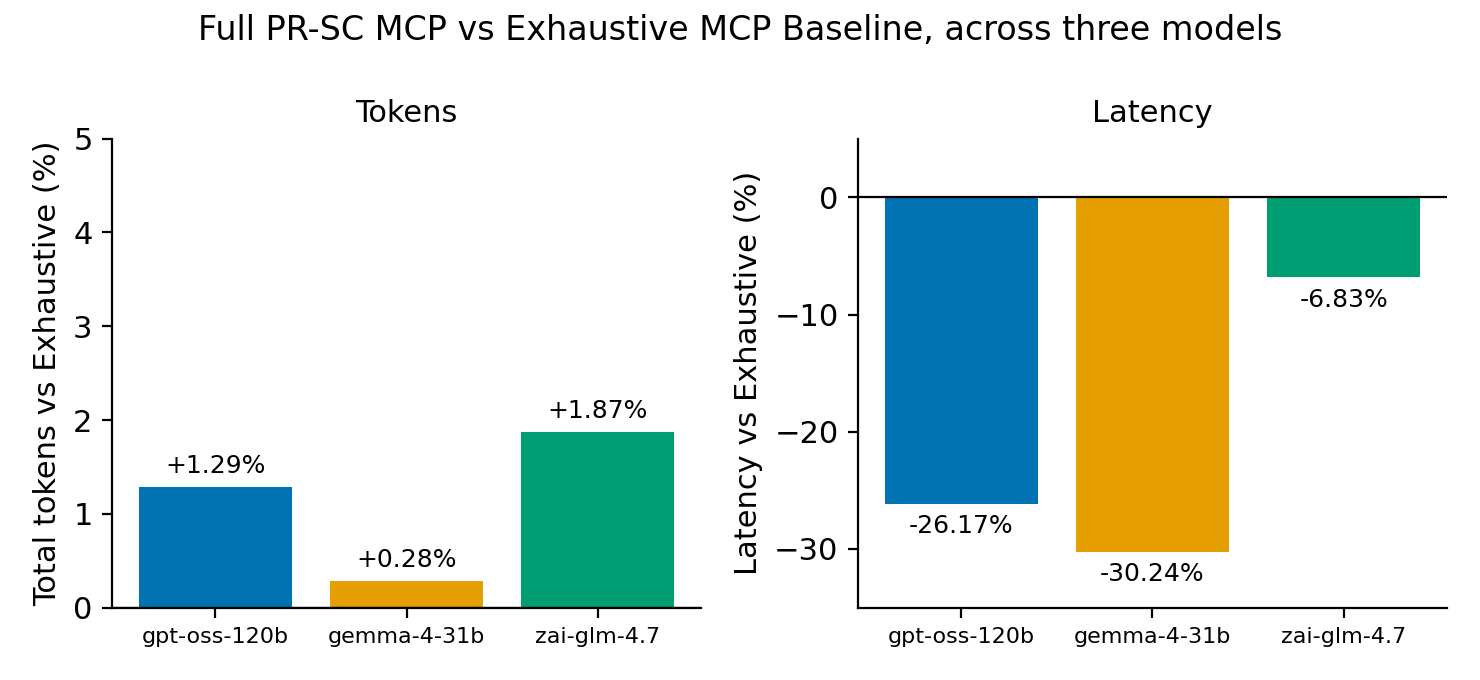
\includegraphics[width=0.8\linewidth]{images/efficiency_chart.png}
\caption{Full PR-SC MCP's token and latency delta versus that model's own Exhaustive MCP Baseline, across all three models. Full PR-SC MCP is near token-neutral on every model, substantially latency-reducing on gpt-oss-120b and gemma-4-31b, and positive but variable on zai-glm-4.7.}
\label{fig:delta}
\end{figure*}

The latency results also show why aggregate means must be interpreted together with run-level stability. On gpt-oss-120b, the five-run latency ranges for the Exhaustive MCP Baseline and Full PR-SC MCP do not overlap (Exhaustive MCP: 769--1121 ms; Full PR-SC MCP: 583--680 ms), supporting a clear and stable latency advantage for Full PR-SC MCP on this model. On gemma-4-31b, Full PR-SC MCP reduced mean latency from 652.1 ms to 454.9 ms (-30.24\%), and the paired run-level confidence interval remains entirely below zero, supporting a clear mean-latency reduction. On zai-glm-4.7, Full PR-SC MCP reduced mean latency from 1919.6 ms to 1788.5 ms (-6.83\%), but the paired run-level interval crosses zero. The appropriate interpretation for zai-glm-4.7 is therefore a favorable but statistically uncertain mean latency reduction, rather than statistically separated dominance.

Taken together, these findings complement the deterministic Architecture Validation results. Architecture Validation shows that PR-SC MCP reduces context burden, tool calls and simulated latency under controlled scoring. Live Validation shows that the same architecture remains near token-neutral under actual generation and produces favorable latency effects when each model is compared with its own exhaustive baseline. The two validation stages therefore support different but compatible claims: Architecture Validation isolates the mechanism, while Live Validation tests whether the mechanism remains operationally plausible under live model behavior.

\FloatBarrier
\subsection{Statistical Interpretation of Live-Generation Results}

Because Live Validation uses the same 10-case $\times$ 4-variant matrix across five independent run batches for each model, the most appropriate uncertainty estimate is computed at the run-batch level rather than by treating the 50 individual generations per variant as independent. For each model and run batch, the mean latency and mean token count of Full PR-SC MCP were subtracted from that model's own Exhaustive MCP Baseline. The resulting five paired run-level differences were then summarized with a two-sided 95\% confidence interval using a $t$ interval with four degrees of freedom. This analysis estimates uncertainty around the architectural contrast while avoiding pseudo-replication at the individual case level.

This framework deliberately prioritizes statistical rigor over statistical power. The individual generations are not treated as fully independent replicates because they are nested within repeated batches, fixed case definitions, and repeated architecture variants. We employ paired run-level aggregation as the primary analysis because the study design includes five repeated live batches per model, and because the resulting Full-vs-baseline differences are transparent, directly tied to the repeated-run design, and less likely to overstate precision. This choice necessarily trades some statistical power for interpretability: with only five paired differences per model, the resulting intervals are wide relative to what a larger repeated-run design would support, but they remain tied directly to the actual repeated-run structure of Live Validation rather than to an independence assumption the design does not satisfy.

\begin{table*}[!t]
  \caption{Run-level confidence intervals for Full PR-SC MCP minus Exhaustive MCP in Live Validation.}
  \label{tab:ci}
  \small
  \begin{tabular}{llccl}
    \toprule
    \textbf{Model} & \textbf{Metric} & \shortstack{\textbf{Mean Full}\\\textbf{$-$ Exhaustive}} & \textbf{95\% CI} & \textbf{Interpretation} \\
    \midrule
    gpt-oss-120b & Latency difference, ms & $-224.66$ & [$-444.69$, $-4.63$] & Latency-reducing \\
    gpt-oss-120b & Total token difference & $12.54$ & [$1.12$, $23.96$] & Small but statistically detectable increase \\
    gemma-4-31b & Latency difference, ms & $-197.18$ & [$-355.67$, $-38.69$] & Latency-reducing \\
    gemma-4-31b & Total token difference & $+1.80$ & Not computable (zero variance) & Identical token count every run (see note) \\
    zai-glm-4.7 & Latency difference, ms & $-131.16$ & [$-304.46$, $42.14$] & Favorable mean, variable by run \\
    zai-glm-4.7 & Total token difference & $+27.10$ & [$-16.64$, $70.84$] & Near token-neutral \\
    \bottomrule
  \end{tabular}
\end{table*}

The interval estimates support the qualitative interpretation used throughout the paper. For gpt-oss-120b, the latency interval remains entirely below zero, supporting a clear mean-latency improvement; its token interval is small in absolute terms (12.5 tokens, about 1.3\% of the baseline) but does not cross zero, indicating a small but statistically detectable increase rather than token-neutrality. For the gemma-4-31b evaluation set, the latency interval also remains entirely below zero, supporting a clear mean-latency improvement. Its token comparison is degenerate rather than merely narrow: because the paired differences have zero sample variance (Table \ref{tab:efficiency}, Note), the resulting interval collapses to a single point ($[+1.80, +1.80]$) and is reported in Table \ref{tab:ci} as not computable rather than as a precise 1.8-token effect. For the zai-glm-4.7 evaluation set, the mean latency difference is favorable to Full PR-SC MCP, but its interval encompasses zero; the data therefore fails to reject the null hypothesis of equal latency at the 95\% confidence level, meaning the result is best interpreted as a positive but statistically uncertain mean latency reduction; its token interval genuinely crosses zero and supports a token-neutral reading. Token behavior therefore differs by model: a small but statistically detectable increase for gpt-oss-120b, a non-computable comparison for gemma-4-31b, and genuine neutrality for zai-glm-4.7.

Operationally, this means that the strongest live efficiency claim is not universal acceleration. The defensible claim is that Full PR-SC MCP preserves deterministic evidence-use indicators, keeps token overhead small, and produces model-dependent latency effects: clear improvement for gpt-oss-120b and gemma-4-31b, and positive but statistically uncertain mean improvement for zai-glm-4.7.

\subsection{Quality and Robustness Across Three Models}

All generated answers were scored using the same deterministic quality and robustness checks: required-tool recall, explicit uncertainty handling, correct stale-versus-fresh evidence prioritization, correct security-distractor handling, and overclaim risk. Required-tool recall specifically checks whether every tool marked as required in a case's definition (Section 3.1) was in fact called by the variant under test, independent of whether that tool's output was ultimately used correctly in the final answer; it is therefore a check on tool-selection behavior rather than on answer quality. Required-tool recall was 1.00 for every model and architecture variant. Uncertainty handling, stale-versus-fresh evidence prioritization, and security-distractor handling reached 100\% across all configurations.

\begin{table*}[!t]
  \caption{Live Validation deterministic quality and robustness checks, across all four variants combined, by model.}
  \label{tab:robustness}
  \small
  \begin{tabular}{lccc}
    \toprule
    \textbf{Metric} & \textbf{gpt-oss} & \textbf{gemma} & \textbf{zai-glm} \\
    \midrule
    Required-tool recall & 1.00 & 1.00 & 1.00 \\
    Uncertainty stated when required & 100\% & 100\% & 100\% \\
    Correct stale-vs-fresh prioritization & 100\% & 100\% & 100\% \\
    Correct security-distractor handling & 100\% & 100\% & 100\% \\
    Overclaim-risk flags & 7 of 20 & 0 of 20 & 0 of 20 \\
    \bottomrule
  \end{tabular}
\end{table*}

Overclaim risk was 0\% for gemma-4-31b and zai-glm-4.7 across all five runs, but was triggered on 7 of 20 dedicated overclaim-risk opportunities for gpt-oss-120b. This variance was strictly concentrated within the single test case featuring a deliberately unavailable required tool; the denominator therefore represents this specific missing-tool scenario across five runs and four architecture variants, rather than the global generation pool. This localized, model-specific deviation highlights a sensitivity of gpt-oss-120b to unresolvable tool dependencies under live-validation constraints.

The binary injection\_safe flag is not interpreted as a direct semantic failure indicator in the dedicated prompt-injection scenario. Generated answers generally identified the malicious instruction and recommended sanitization or trusted-source verification. Consequently, prompt-injection handling is evaluated as a qualitative diagnostic check rather than by relying solely on the binary flag.

\subsection{Semantic Review and Validation Summary}

To complement deterministic post-checks, we conducted a semantic review on a stratified sample of 60 generated answers. The sample covered three models, four architecture variants, and five diagnostically relevant case families: latency degradation, conflicting evidence, prompt injection in tool output, missing required tool, and stale data. These five were selected out of the ten Live Validation case families specifically because each depends on a judgment call that a deterministic check can only approximate: whether conflicting or stale evidence was weighted correctly, whether a missing tool was handled without overclaiming, and whether the model's explanation of an injected instruction was actually sound rather than merely containing the right keywords. To ensure maximum objectivity, the scoring was conducted via a blinded design by a domain-expert reviewer. The reviewer was shown only the controlled evidence, the generated answer, the case identifier and the case family; model identity, architecture variant, source file and run identifier were withheld during scoring.

Each answer was scored on a 1--5 rubric covering faithfulness, completeness, causal discipline, evidence prioritization and actionability. The review matched the preliminary rubric-based scores prepared before unblinding. Across variants, mean semantic scores remained high and tightly clustered, with no evidence that Full PR-SC MCP degraded answer quality relative to Exhaustive MCP Baseline or the routing-only variants. This supports the interpretation that PR-SC MCP's efficiency gains and context-governance behavior do not come at the cost of human-reviewed semantic quality in the evaluated sample.

\begin{table*}[!t]
  \caption{Semantic review scores by architecture variant. Scores are averaged across a stratified 60-answer review sample. Model and variant labels were withheld during scoring and restored only for aggregation.}
  \label{tab:semantic}
  \begin{tabular}{lcccccc}
    \toprule
    \textbf{Variant} & \textbf{Responses} & \textbf{Faithfulness} & \textbf{Completeness} & \shortstack{\textbf{Causal}\\\textbf{discipline}} & \shortstack{\textbf{Evidence}\\\textbf{prioritization}} & \textbf{Actionability} \\
    \midrule
    Exhaustive MCP & 15 & 5.00 & 5.00 & 4.67 & 5.00 & 5.00 \\
    Routing MCP & 15 & 5.00 & 5.00 & 4.60 & 4.87 & 5.00 \\
    Routing + Packaging & 15 & 5.00 & 5.00 & 4.80 & 5.00 & 5.00 \\
    Full PR-SC MCP & 15 & 5.00 & 5.00 & 4.67 & 5.00 & 5.00 \\
    \bottomrule
  \end{tabular}
\end{table*}

The review should be interpreted as a calibration layer rather than a complete replacement for deterministic scoring or a full human evaluation of all live generations. Nevertheless, its agreement with the preliminary rubric-based scores increases confidence that the deterministic evidence-use checks are directionally aligned with semantic answer quality, and that Full PR-SC MCP preserves human-reviewed answer quality in the evaluated sample.

Table \ref{tab:summary} places Full PR-SC MCP's efficiency profile relative to Exhaustive MCP side by side across both validation stages. The token-reduction advantage is substantial under the controlled Architecture Validation framework; under live generation across three independent models it narrows, as expected once a live model's own generation behavior is in the loop, but it does not turn into a material token penalty. Full PR-SC MCP remains near token-neutral across all three models, substantially reduces mean latency for gpt-oss-120b and gemma-4-31b, and shows a positive but statistically uncertain mean latency reduction for zai-glm-4.7. This is the central empirical argument for the two-stage methodology adopted in Section 3: a controlled benchmark can show what an architecture is capable of, but only live, repeated, multi-model testing can show whether that capability holds up in practice.

\begin{table*}[!t]
  \caption{Full PR-SC MCP's efficiency delta versus Exhaustive MCP, across Architecture Validation and each of the three Live Validation models.}
  \label{tab:summary}
  \begin{tabular}{p{0.24\linewidth}p{0.30\linewidth}p{0.36\linewidth}}
    \toprule
    \textbf{Stage / Model} & \textbf{Condition} & \textbf{Full PR-SC MCP vs Exhaustive} \\
    \midrule
    Architecture Validation & Controlled + semi-real, deterministic scoring & $-47.1\%$ tokens, $-27.4\%$ latency \\
    Live Validation --- gpt-oss-120b & Live generation, 5-run mean & $+1.29\%$ tokens, $-26.17\%$ latency \\
    Live Validation --- gemma-4-31b & Live generation, 5-run mean & $+0.28\%$ tokens, $-30.24\%$ latency \\
    Live Validation --- zai-glm-4.7 & Live generation, 5-run mean & $+1.87\%$ tokens, $-6.83\%$ latency \\
    \bottomrule
  \end{tabular}
\end{table*}

\section{DISCUSSION}

The deterministic Architecture Validation results from the controlled framework support Full PR-SC MCP as the strongest complete quality-efficiency configuration under controlled scoring. Live Validation asks whether that conclusion survives contact with an actual model, and across three independent open-weight models it does in a bounded but useful form: Full PR-SC MCP remains near token-neutral relative to Exhaustive MCP, substantially reduces mean latency for gpt-oss-120b and gemma-4-31b, and shows a positive but statistically uncertain mean latency reduction for zai-glm-4.7. The blinded domain-expert semantic review further supports the interpretation that these efficiency and context-governance benefits do not come at the cost of reviewed semantic answer quality in the evaluated sample. The study's discipline of exposing quality, efficiency, grounding, robustness, live-generation behavior, and human-calibrated semantic review together, across more than one model rather than collapsing them into a single number from a single run, is what allows this conclusion to be reported with more confidence than a single benchmark run could support.

Viewed this way, PR-SC MCP is best understood as an integration of established ideas rather than as a rejection of prior work. MCP provides the connectivity layer, retrieval and Self-RAG motivate evidence grounding, long-context research motivates salience-aware packaging, Toolformer, ReAct and Gorilla motivate tool use and tool selection, compression research motivates controlled context reduction, and agent benchmarks motivate systematic evaluation. The contribution of this paper is to connect these ideas inside a single MCP-specific context lifecycle and to test the resulting trade-offs across controlled, live, and human-calibrated evaluation layers.

\subsection{Claim Boundary}

The study supports the claim that PR-SC MCP is a viable context-governance architecture, validated under controlled and semi-real conditions and consistently confirmed across three independent open-weight models under live generation. It does not support production deployment readiness, since operational realism beyond the synthetic and semi-real evidence used here remains untested, and it does not support a claim of universal cost optimality across every possible model or provider, since only three models, all served on the same inference infrastructure, have been tested to date. Table \ref{tab:claims} summarizes the evidentiary strength and boundary of each major claim made across both validation stages.

\begin{table*}[!t]
  \caption{Global claim matrix: strength and boundary of the study's main claims.}
  \label{tab:claims}
  \begin{tabular}{p{0.2\linewidth}p{0.16\linewidth}p{0.12\linewidth}p{0.42\linewidth}}
    \toprule
    \textbf{Claim} & \textbf{Supported by} & \textbf{Strength} & \textbf{Boundary} \\
    \midrule
    Routing reduces unnecessary context & Architecture Validation, Live Validation & Strong & Controlled and live benchmark settings \\
    Compression reduces prompt burden & Architecture Validation & Strong pre-live & Not isolated as a standalone factor in Live Validation \\
    Packaging improves evidence usability & Architecture Validation, Live Validation & Moderate to strong & Needs human calibration for final quality claims \\
    Full PR-SC MCP improves governance without a material live-generation efficiency penalty & Architecture Validation, Live Validation (3 models) & Strong within tested scope & Small token overhead (0.3--1.9\%): statistically detectable rather than neutral for gpt-oss-120b, not computable for gemma-4-31b (Table \ref{tab:ci}), and genuinely neutral for zai-glm-4.7; latency-improving for gpt-oss-120b and gemma-4-31b, but the latency interval encompasses zero for zai-glm-4.7 on shared Cerebras infrastructure \\
    PR-SC MCP is production ready & Not supported & Not applicable & Production-like validation required \\
    Efficiency profile generalizes to every model and provider & Not yet tested beyond three open-weight models on shared infrastructure & Untested & Requires broader multi-model, multi-provider, multi-infrastructure comparison \\
    \bottomrule
  \end{tabular}
\end{table*}

\subsection{Why the Efficiency Result Replicates Across Models}

A reasonable question is why a controlled synthetic benchmark and a semi-real benchmark, evaluated with no live model in the loop, would predict the live-generation outcome as closely as Table \ref{tab:summary} shows. Architecture Validation's deterministic proxies---simulated latency, estimated cost, rule-based accuracy and faithfulness---are computed directly from the architecture's own instrumentation: token counts, tool counts and evidence-retention checks that do not depend on any model's generation behavior. Because routing, compression and packaging act on the context before it ever reaches a model, their token and tool-count effects are largely mechanical rather than model-specific, which is consistent with why three models from three different organizations, evaluated independently, reproduce the same direction of effect. This does not guarantee the same result on every conceivable model---Section 5.1 returns to that boundary---but it explains why this three-model replication is a more informative outcome than it might first appear: the mechanism being tested is upstream of model-specific generation behavior, not downstream of it.

\subsection{Implications for MCP-Agent Evaluation}

Three implications follow for how MCP-based agents should be evaluated going forward. First, a controlled or semi-real benchmark with deterministic scoring is not merely a cheaper proxy for live evaluation; when the mechanisms under test act on context before generation, as routing, compression and packaging do, deterministic scoring can be genuinely predictive of live behavior, and this study's two-stage design is what made that predictiveness checkable rather than assumed. Second, single-model live validation cannot distinguish an architectural effect from a model-specific idiosyncrasy; only evaluating more than one model, under the same case matrix and the same scoring rules, establishes whether an observed pattern is a property of the architecture or of the one model tested. Third, repeated runs per model, not single runs, are necessary even when the architecture-level effect is consistent: individual runs on every model tested here still showed some variability, and it is the five-run mean, not any single pass, that supports the claims in this paper.

\subsection{Practical Guidance for Practitioners}

For a team building an MCP-based agent today, two practical conclusions follow from Sections 4--5. First, adopt routing and compression by default: the token, tool-count and latency gains under Architecture Validation are large, consistent across controlled and semi-real conditions, come with no measured quality cost, and held up across every model tested under live generation. Second, adopt the full packaging and ledgering layer for auditability with reasonable confidence that it will not cost more in live tokens---on the three models tested here it was token-neutral or better---while recognizing that this has been confirmed on open-weight models sharing one inference provider, and re-running at least a small multi-variant matrix like the one in Sections 4.2--4.3 is still worthwhile before relying on the same result on a new model or infrastructure.

\section{LIMITATIONS}

Four limitations bound the current findings. First, all three models tested under Live Validation---gpt-oss-120b, gemma-4-31b and zai-glm-4.7---are open-weight models served on the same Cerebras infrastructure; no closed frontier model and no model served on commodity GPU infrastructure has been tested, so the consistency observed across these three models cannot yet be generalized beyond open-weight models on this specific inference stack. The use of a single serving provider improves internal consistency across the three-model comparison, but it also means that the latency findings should be interpreted as Cerebras-served latency effects rather than as provider-independent infrastructure results. All three models completed the full live-validation matrix, but statistical power remains limited to five run-level repetitions per model; the confidence intervals reported in Section 4.4 therefore quantify uncertainty but should not be over-interpreted as definitive distributional claims. Run-level latency variability remains visible, especially for gemma-4-31b and zai-glm-4.7. Second, the Live Validation benchmark is deliberately controlled and synthetic: this is necessary for causal attribution and repeatability, but it does not substitute for production incident diversity, real user phrasing, provider-side queuing effects, or full end-to-end orchestration cost. Third, the study includes a blinded domain-expert semantic review calibration sample, but not a full human evaluation of all 600 total generations. The human review therefore supports the alignment between deterministic checks and semantic quality but should not be interpreted as exhaustive human assessment. Fourth, the Architecture Validation values reported in this version are generated by deterministic validation framework included with the study; they should be interpreted as the reproducible controlled-runner result associated with the accompanying GitHub materials.

\section{CONCLUSION}

This study set out to answer whether predictive routing, source-aware compression, evidence packaging and an observability feedback loop can improve the efficiency, traceability and robustness of MCP-based LLM agents while preserving answer quality, and whether that answer would survive contact with a live model rather than only deterministic scoring. Architecture Validation gives a positive answer under controlled and semi-real conditions: within the deterministic validation framework accompanying this study, Full PR-SC MCP reduced prompt tokens by 47.1\%, tool calls by 39.1\% and simulated latency by 27.4\% relative to the Exhaustive MCP Baseline, while improving deterministic accuracy and faithfulness to 2.00 on the 0--2 scoring scale.

Live Validation confirms that answer rather than complicating it. Tested across three independent open-weight models---gpt-oss-120b, gemma-4-31b and zai-glm-4.7---each evaluated five times with a single consistent runner script, Full PR-SC MCP remained near token-neutral relative to Exhaustive MCP and preserved deterministic evidence-use indicators. It substantially reduced mean latency for gpt-oss-120b and gemma-4-31b, and the zai-glm-4.7 replication set also shows a favorable mean latency reduction, although with run-level confidence intervals encompassing zero. No model showed a material token penalty and run-level confidence intervals support a model-dependent efficiency claim rather than a universal per-run dominance claim. The blinded domain-expert semantic review calibration further found no evidence that Full PR-SC MCP degraded semantic answer quality in the evaluated sample. This consistency across three independently developed models, run independently and repeatedly, is what allows the Architecture Validation result to be reported as a property of the architecture rather than as an artifact of controlled scoring or of any single model's behavior.

Taken together, the two validation stages support a single, disciplined claim: MCP-based agents benefit from explicit context governance---routing, compression, ledgering and packaging---under controlled conditions, and that benefit persists, consistently, under live generation across multiple independent models. Scalable MCP-based agents therefore need more than access to external tools: they need disciplined, observable governance over which evidence is selected, how it is transformed, how it is ordered for the model, and how the resulting behavior is measured, repeatedly and across more than one model, before that governance can be trusted.

\section*{Data and Code Availability}

\begin{sloppypar}
Per-run records, per-variant summaries and generated-answer transcripts for Live Validation (Sections 4.2--4.6), in CSV and JSON form, are listed in the reproducibility manifest of the accompanying technical supplement. The live-validation runner used for every model in this study, \texttt{v5\_1\allowbreak\_cerebras\allowbreak\_subset\allowbreak\_runner\allowbreak\_v1.py}, will be released publicly in the accompanying repository at submission. The regenerated Architecture Validation runner, \texttt{pr\_sc\allowbreak\_mcp\allowbreak\_architecture\allowbreak\_validation\allowbreak\_runner.py}, is included as a deterministic implementation of the documented 24-case $\times$ 8-variant controlled/semi-real protocol and is the source of the Architecture Validation values reported in Table \ref{tab:archval}. Case definitions and ground truth for Architecture Validation (Section 4.1) are embedded in that runner and documented in the technical supplement's methodology chapters.
\end{sloppypar}
